% ════════════════════════════════════════════════════════════════
%  CHAPITRE 2 — ÉTAT DE L'ART ET CHOIX TECHNOLOGIQUES
% ════════════════════════════════════════════════════════════════

\chapter{État de l'art et choix technologiques}
\graphicspath{{Isipfe/Figures/}{diagramms/}}

% ── Introduction du chapitre ────────────────────────────────────
\section*{Introduction}
\addcontentsline{toc}{section}{Introduction}

Ce chapitre analyse les solutions de recrutement existantes, justifie les
choix technologiques retenus et présente l'architecture globale de la
plateforme.

% ════════════════════════════════════════════════════════════════
\section{État de l'art}
% ════════════════════════════════════════════════════════════════

\subsection{Présentation du domaine}

Le recrutement numérique repose aujourd'hui sur des outils appelés
\textit{Applicant Tracking Systems} (ATS), ou systèmes de suivi des
candidatures. Leur rôle est de centraliser les offres d'emploi, la
réception des candidatures, le tri des profils et le suivi des étapes
jusqu'à la décision finale.

Ces outils améliorent la traçabilité et réduisent le travail manuel des
équipes RH. Dans notre contexte, l'enjeu n'est pas seulement d'adopter un
ATS, mais de construire une solution réellement adaptée à l'organisation
multi-sites de Schulte Automotive Tunisia.

\subsection{Solutions existantes}

Nous avons étudié quatre familles de solutions :
\begin{itemize}
    \item les ATS \textbf{SaaS Enterprise} (ex. Workday, Taleo) ;
    \item les ATS \textbf{SaaS PME} (ex. Greenhouse, Lever) ;
    \item les solutions \textbf{open source} (ex. OpenCATS) ;
    \item les \textbf{portails d'emploi} généralistes (ex. LinkedIn,
    Emploi.tn).
\end{itemize}

Chaque famille apporte des avantages, mais aucune ne couvre complètement
les contraintes locales, organisationnelles et budgétaires du projet.

\subsection{Étude comparative}

\begin{table}[H]
\centering
\caption{Étude comparative des solutions existantes}
\begin{tabularx}{\textwidth}{|l|l|X|X|}
\hline
\textbf{Solution} & \textbf{Type} & \textbf{Points forts} & \textbf{Limites} \\
\hline
Workday / Taleo & SaaS Enterprise & Très complet, mature, intégré &
Coût élevé, lourd à déployer, peu flexible localement \\
\hline
Greenhouse / Lever & SaaS PME & Interface moderne, usage simple &
Payant, isolation multi-site limitée \\
\hline
OpenCATS & Open source & Gratuit, auto-hébergeable &
Fonctionnalités limitées, maintenance irrégulière \\
\hline
Portails d'emploi & Plateforme publique & Bonne visibilité des offres &
Pas de workflow RH interne complet \\
\hline
Solution proposée & Sur mesure & Adaptée au besoin réel, maîtrise totale &
Temps initial de développement plus long \\
\hline
\end{tabularx}
\end{table}

\subsection{Limites}

L'analyse met en évidence quatre limites principales des solutions
existantes dans notre cas :
\begin{itemize}
    \item coût parfois trop élevé pour un déploiement local ;
    \item personnalisation insuffisante du workflow RH ;
    \item faible prise en charge de l'isolation entre sites ;
    \item adaptation partielle au contexte tunisien.
\end{itemize}

Ces limites justifient un développement sur mesure.

À partir de ce constat, la section suivante détaille les choix techniques
retenus pour transformer ces limites en décisions concrètes.

% ════════════════════════════════════════════════════════════════
\section{Choix technologiques}
% ════════════════════════════════════════════════════════════════

\subsection{Critères de choix}

Nos choix techniques ont été guidés par les critères suivants :
\begin{itemize}
    \item simplicité de maintenance ;
    \item performance et stabilité ;
    \item sécurité et traçabilité ;
    \item compatibilité mobile ;
    \item cohérence de la pile technique (TypeScript de bout en bout).
\end{itemize}

\subsection{Technologies retenues}

\subsubsection{Backend}

Le backend est basé sur \textbf{Node.js}, \textbf{Express} et
\textbf{TypeScript}. Cette combinaison permet de construire une API REST
claire, évolutive et facile à maintenir.

Pour la communication temps réel (notifications, changements de statut),
nous utilisons \textbf{Socket.io}.

\subsubsection{Frontend}

La partie frontend est divisée en trois interfaces :
\begin{itemize}
    \item \textbf{PWA candidat} avec \textbf{Next.js} ;
    \item \textbf{interface RH} avec \textbf{React + Vite} ;
    \item \textbf{interface Admin} avec \textbf{React + Vite}.
\end{itemize}

Ce choix permet d'offrir une expérience mobile fluide côté candidat,
et un environnement rapide côté interne (RH et admin).

\subsubsection{Base de données}

Nous avons retenu \textbf{PostgreSQL} pour le stockage des données, et
\textbf{Prisma} comme ORM.

PostgreSQL apporte robustesse et fiabilité transactionnelle. Prisma,
quant à lui, facilite les migrations, la cohérence du schéma et la
sécurité des accès aux données.

\subsubsection{Outils DevOps}

Les principaux outils DevOps utilisés sont :
\begin{itemize}
    \item \textbf{Git / GitHub} pour le versionnement ;
    \item \textbf{npm} pour la gestion des dépendances et scripts ;
    \item \textbf{Prisma Migrate} pour le versionnement du schéma BD ;
    \item \textbf{curl} et \textbf{Vitest} pour les tests API et unitaires ;
    \item \textbf{Overleaf} pour la collaboration sur le rapport.
\end{itemize}

\subsection{Justification des choix}

Les technologies retenues répondent bien à nos besoins :
\begin{itemize}
    \item elles sont connues, documentées et maintenues ;
    \item elles réduisent la complexité de développement ;
    \item elles permettent une architecture modulaire ;
    \item elles facilitent l'évolution future de la plateforme.
\end{itemize}

En pratique, ce socle technique offre un bon équilibre entre performance,
coût et maintenabilité.

La dernière section relie ces choix à la structure réelle du système,
à travers la vue d'architecture et les composants principaux.

% ════════════════════════════════════════════════════════════════
\section{Architecture du système}
% ════════════════════════════════════════════════════════════════

\subsection{Type d'architecture}

Le système suit une \textbf{architecture en couches} (présentation,
logique métier, données) avec un backend central partagé par les trois
interfaces.

Ce modèle améliore la séparation des responsabilités et simplifie la
maintenance.

Dans cette architecture, les applications frontend jouent le rôle de
\textit{consommateurs d'API} : elles appellent les services HTTP du
backend, tandis que les mises à jour temps réel sont propagées via Socket.
Ce positionnement confirme une architecture client--serveur centralisée,
plutôt qu'une approche microservices.

\subsection{Schéma global}

La figure suivante présente la vue globale de l'architecture.

\begin{figure}[H]
\centering
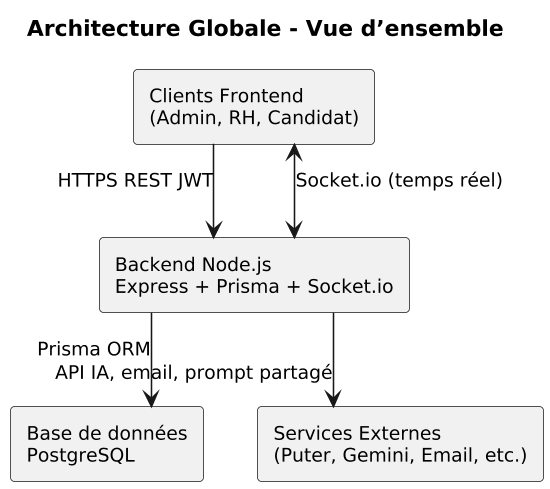
\includegraphics[width=0.90\textwidth]{architecture_globale}
\caption{Schéma global de l'architecture de la plateforme}
\end{figure}

Ce schéma se lit de gauche à droite : interfaces utilisateur (candidat,
RH, admin), services backend (API et temps réel), puis couche de données.
Cette lecture met en évidence la séparation des responsabilités, le point
de contrôle unique de la logique métier, et la centralisation des données.

Le backend ne pilote pas les interfaces par requêtes directes ; il expose
des endpoints consommés par les clients, puis notifie les changements
d'état par événements temps réel.

\subsection{Description des composants}

\begin{table}[H]
\centering
\caption{Composants principaux du système}
\begin{tabularx}{\textwidth}{|l|l|X|}
\hline
\textbf{Composant} & \textbf{Technologie} & \textbf{Rôle} \\
\hline
PWA candidat & Next.js & Consulter les offres, postuler, suivre la candidature \\
\hline
Interface RH & React + Vite & Gérer les offres, candidatures et entretiens \\
\hline
Interface Admin & React + Vite & Gérer les comptes RH et modèles d'offres \\
\hline
Backend API & Node.js + Express & Authentification, logique métier, exposition REST \\
\hline
Temps réel & Socket.io & Notifications et mises à jour instantanées \\
\hline
Base de données & PostgreSQL + Prisma & Stockage, requêtes et intégrité des données \\
\hline
\end{tabularx}
\end{table}

% ── Conclusion du chapitre ──────────────────────────────────────
\section*{Conclusion du chapitre 2}
\addcontentsline{toc}{section}{Conclusion du chapitre 2}

Ce chapitre a permis de relier trois niveaux d'analyse : les limites des
solutions existantes, les choix technologiques qui en découlent, puis leur
traduction dans une architecture cohérente.

Le chapitre suivant s'appuie sur ce socle pour formaliser les besoins et
la modélisation UML du système.
